
\documentclass[11pt]{article}
\usepackage[utf8]{inputenc}
\usepackage[margin=1in]{geometry}
\usepackage{graphicx}
\usepackage{booktabs}
\usepackage{xcolor}
\usepackage{hyperref}

\definecolor{primary}{RGB}{44, 62, 80}
\definecolor{secondary}{RGB}{231, 76, 60}

\title{\vspace{-2cm}\color{primary}\textbf{Fund of Hedge Funds Strategy Overview}}
\author{}
\date{\vspace{-1.5cm}}

\begin{document}
\maketitle

\section*{\color{primary}Overview}
This product is a fund of hedge funds. The core idea is to pick strong performers that are uncorrelated, ensuring that returns keep up while overall volatility and max drawdown are significantly reduced. By blending distinct, non-overlapping strategies, the portfolio aims for robust risk-adjusted returns across market cycles.

\section*{\color{primary}Fund Allocation \& Strategy Descriptions}
The table below highlights the initial capital allocation weights alongside a brief description of each underlying fund's distinct edge and methodology.

\begin{itemize}
    \item \textbf{Quanstream}: Volatility seller across more than 150 commodities underlying with over 20 years of experience in these strategies.
    \item \textbf{M1}: Crypto carry trade market neutral fund.
    \item \textbf{Vadantia}: Trading-oriented fund on FX and precious metals with more than 4 trades per day.
    \item \textbf{Wizard Quant}: Chinese equity market neutral fund that is strictly quant-driven.
    \item \textbf{ARR}: Trading fund on equities and macro, utilizing a quantamental approach to identify equities with high upside, backed by a strict risk management policy.
    \item \textbf{R Squared}: Equities futures arbitrage and dividend futures arbitrage relative value style fund.
    \item \textbf{Shiprock}: Fund investing in highly distressed debt and bond contracts.
    \item \textbf{Smithson}: Smithson fund description.
    \item \textbf{26 Miles}: Indian-based fund investing in medium-frequency strategies across a lot of asset classes (intra-day trading with holdings of 2-3 hours). Founded by a team with strong prop trading desk experience who spun out to create this fund.
    \item \textbf{Adar1}: Adar1 fund description.
    \item \textbf{Sam Capital}: Sam capital fund description.
\end{itemize}


\section*{\color{primary}Performance \& Correlation}
The following visuals illustrate the fund-level statistics and the diversification benefits.

\begin{figure}[h]
    \centering
    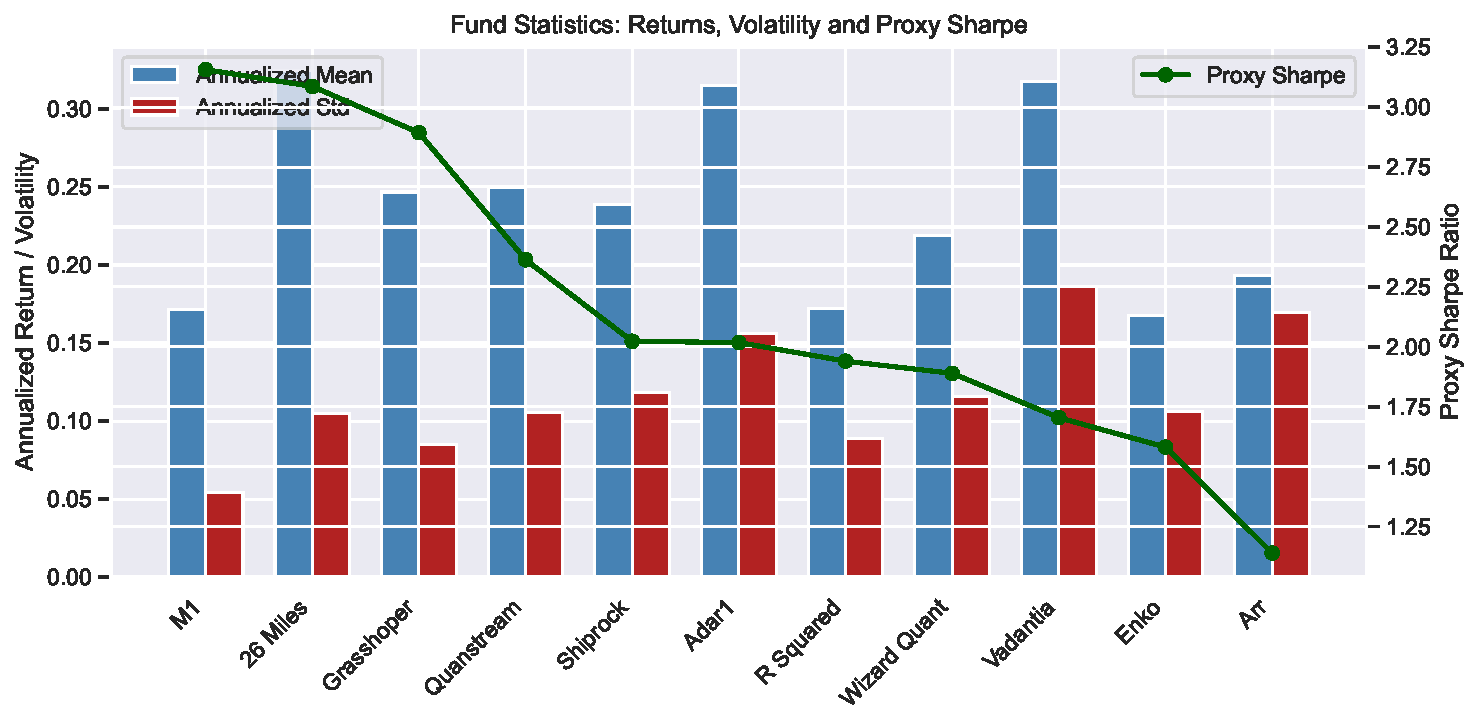
\includegraphics[width=0.8\textwidth]{fund_stats.pdf}
\end{figure}

\begin{figure}[h]
    \centering
    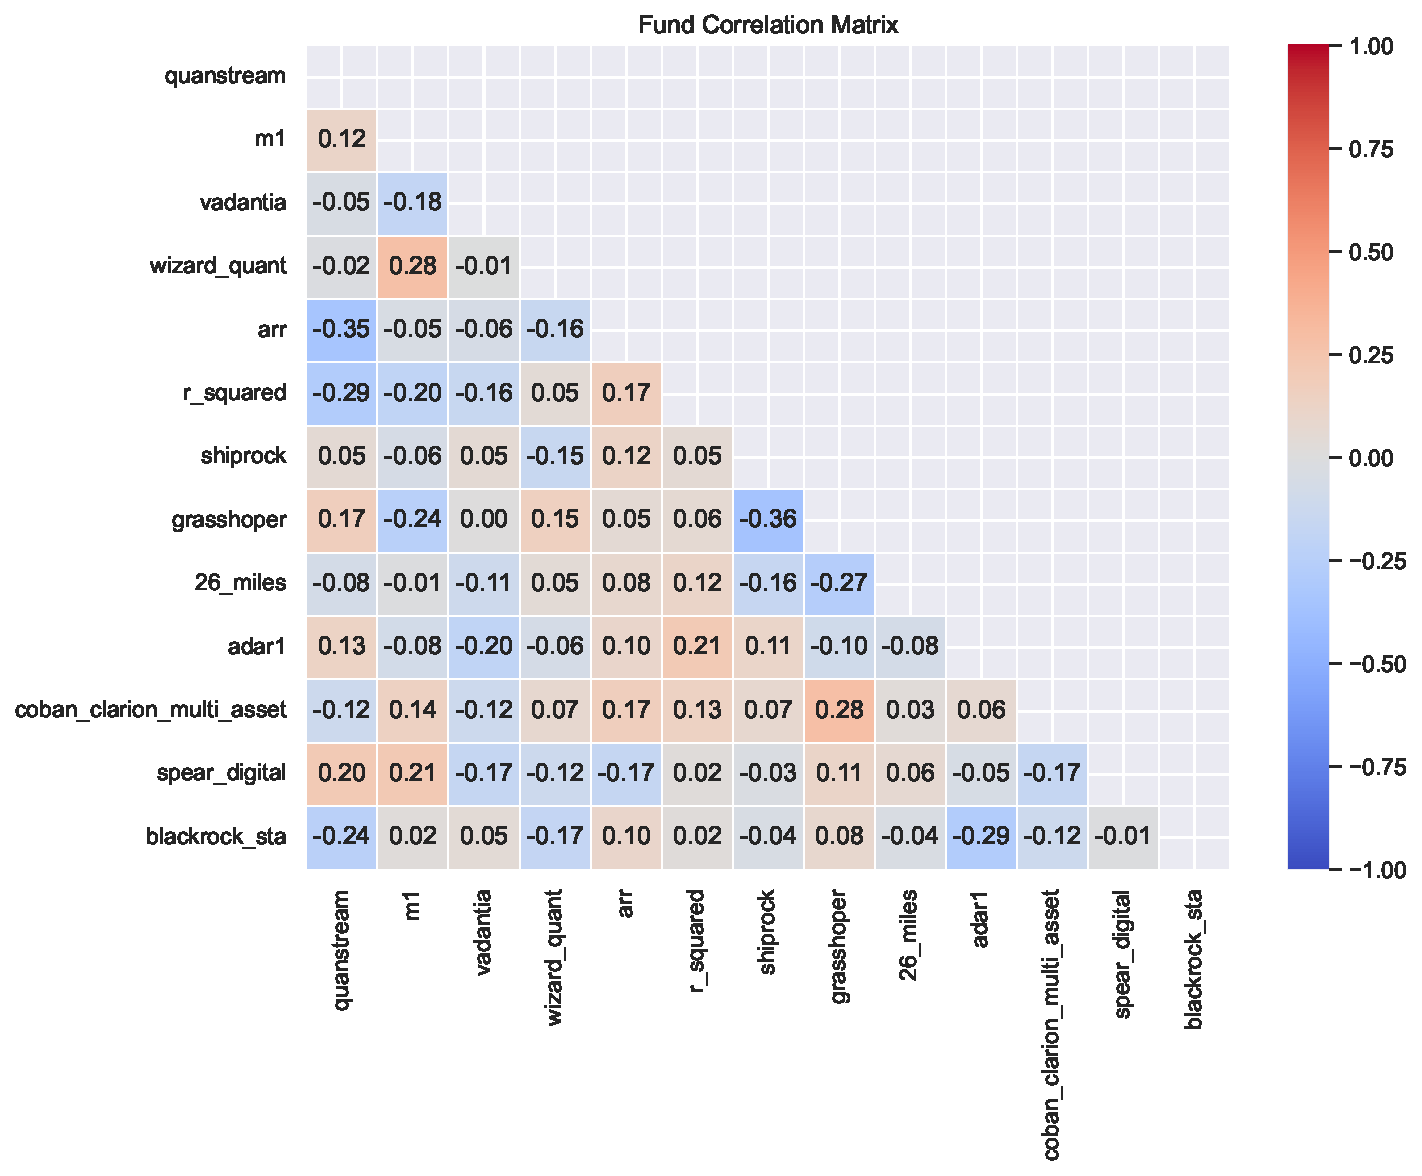
\includegraphics[width=0.7\textwidth]{correlation.pdf}
\end{figure}

\begin{figure}[h]
    \centering
    
\includegraphics[width=0.9\textwidth]{worst_sp500_months.pdf}
\end{figure}

\clearpage
\section*{\color{primary}Detailed Fund Statistics}
\begin{table}[h]
\centering
\resizebox{\textwidth}{!}{%
\begin{tabular}{lccccccccccccc}
\toprule
 & \textbf{CAGR} & \textbf{Std} & \textbf{Proxy Sharpe} & \textbf{MDD} & \textbf{Calmar} & \textbf{Pos Months} & \textbf{Up Capture} & \textbf{Down Capture} & \textbf{Alpha (t-stat)} & \textbf{Beta} & \textbf{Corr SP500} & \textbf{N months}\\
\midrule
\textbf{Quanstream} & 21.50\% & 8.46\% & 2.36 & -9.18\% & 2.34 & 78.6\% & 0.51 & -0.36 & 18.82\% (9.26) & 0.09 & 0.17 & 215 \\
\textbf{M1} & 18.37\% & 5.43\% & 3.16 & -0.77\% & 23.91 & 92.5\% & 0.43 & -0.41 & 15.81\% (4.79) & 0.06 & 0.15 & 40 \\
\textbf{Vadantia} & 34.62\% & 18.63\% & 1.70 & -26.03\% & 1.33 & 69.6\% & 0.68 & -0.75 & 34.33\% (5.44) & -0.17 & -0.14 & 112 \\
\textbf{Wizard Quant} & 20.55\% & 13.63\% & 1.45 & -10.84\% & 1.90 & 65.2\% & 0.39 & -0.60 & 20.53\% (4.86) & -0.06 & -0.06 & 135 \\
\textbf{Arr} & 19.54\% & 16.97\% & 1.14 & -15.68\% & 1.25 & 59.6\% & 0.55 & -0.16 & 18.44\% (2.19) & 0.07 & 0.07 & 52 \\
\textbf{R Squared} & 18.18\% & 8.86\% & 1.94 & -4.78\% & 3.80 & 71.2\% & 0.48 & -0.16 & 15.35\% (3.80) & 0.13 & 0.24 & 59 \\
\textbf{Shiprock} & 25.85\% & 11.81\% & 2.02 & -8.74\% & 2.96 & 78.1\% & 0.68 & -0.03 & 20.12\% (4.08) & 0.19 & 0.26 & 73 \\
\textbf{Smithson} & 47.17\% & 6.69\% & 5.90 & -0.63\% & 74.87 & 96.9\% & 0.80 & -1.00 & 40.02\% (13.31) & -0.04 & -0.08 & 65 \\
\textbf{26 Miles} & 24.90\% & 7.36\% & 3.09 & -2.20\% & 11.33 & 84.4\% & 0.44 & -0.62 & 24.14\% (7.39) & -0.10 & -0.20 & 64 \\
\textbf{Adar1} & 34.92\% & 15.60\% & 2.02 & -10.63\% & 3.28 & 74.4\% & 0.88 & -0.18 & 26.38\% (4.60) & 0.31 & 0.34 & 86 \\
\textbf{Sam Capital} & 47.02\% & 14.44\% & 2.78 & -15.19\% & 3.10 & 86.8\% & 1.16 & -0.57 & 36.15\% (10.11) & 0.28 & 0.28 & 197 \\
\bottomrule
\end{tabular}
}
\end{table}

\section*{\color{primary}Portfolio Growth Analysis}
Here we compare four portfolio weighting methodologies.

\begin{figure}[h]
    \centering
    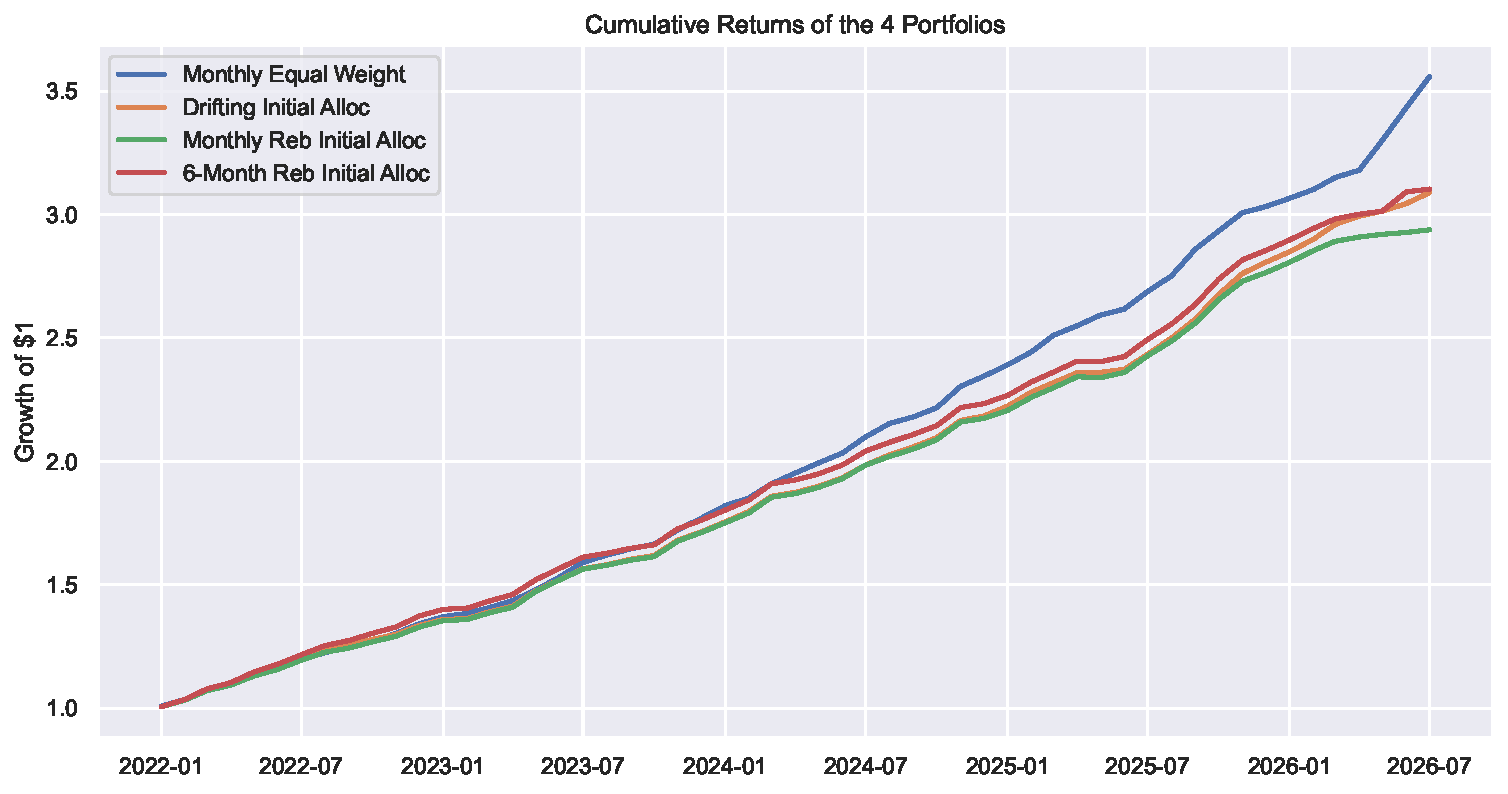
\includegraphics[width=\textwidth]{4_strategies_growth.pdf}
\end{figure}

\clearpage
\section*{\color{primary}6-Month Rebalancing Strategy Deep-Dive}
The 6-Month Rebalancing Strategy resets the allocations back to target weights bi-annually, capturing drift while avoiding excessive turnover costs.

\subsection*{Strategy Statistics}
\begin{table}[h]
\centering
\resizebox{\textwidth}{!}{%
\begin{tabular}{lccccccccccccc}
\toprule
 & \textbf{CAGR} & \textbf{Std} & \textbf{Proxy Sharpe} & \textbf{MDD} & \textbf{Calmar} & \textbf{Pos Months} & \textbf{Up Capture} & \textbf{Down Capture} & \textbf{Alpha (t-stat)} & \textbf{Beta} & \textbf{Corr SP500} & \textbf{N months}\\
\midrule
\textbf{6-Month Rebalanced} & 29.82\% & 3.38\% & 7.83 & 0.00\% & - & 100.0\% & 0.62 & -0.45 & 26.00\% (15.72) & 0.04 & 0.17 & 52 \\
\bottomrule
\end{tabular}
}
\end{table}

\subsection*{Monthly Returns Breakdown}
\begin{table}[h]
\centering
\resizebox{\textwidth}{!}{%
\begin{tabular}{lccccccccccccc}
\toprule
\textbf{Year} & \textbf{Jan} & \textbf{Feb} & \textbf{Mar} & \textbf{Apr} & \textbf{May} & \textbf{Jun} & \textbf{Jul} & \textbf{Aug} & \textbf{Sep} & \textbf{Oct} & \textbf{Nov} & \textbf{Dec} & \textbf{YTD} \\
\midrule
2022 & 0.3\% & 2.6\% & 3.6\% & 2.2\% & 3.6\% & 2.8\% & 3.6\% & 3.3\% & 2.0\% & 2.5\% & 2.1\% & 3.4\% & 37.1\% \\
2023 & 2.1\% & 0.6\% & 2.1\% & 2.0\% & 4.1\% & 2.9\% & 2.9\% & 1.2\% & 1.3\% & 1.0\% & 3.8\% & 2.2\% & 29.5\% \\
2024 & 2.4\% & 2.2\% & 3.6\% & 1.1\% & 1.5\% & 1.9\% & 2.8\% & 1.8\% & 1.6\% & 1.8\% & 3.4\% & 0.9\% & 28.0\% \\
2025 & 1.6\% & 2.3\% & 1.9\% & 2.0\% & 0.2\% & 1.1\% & 3.0\% & 2.5\% & 3.2\% & 3.9\% & 2.8\% & 1.5\% & 29.2\% \\
2026 & 1.6\% & 1.6\% & 1.4\% & 0.8\% & - & - & - & - & - & - & - & - & 5.6\% \\
\bottomrule
\end{tabular}
}
\end{table}

\begin{figure}[h]
    \centering
    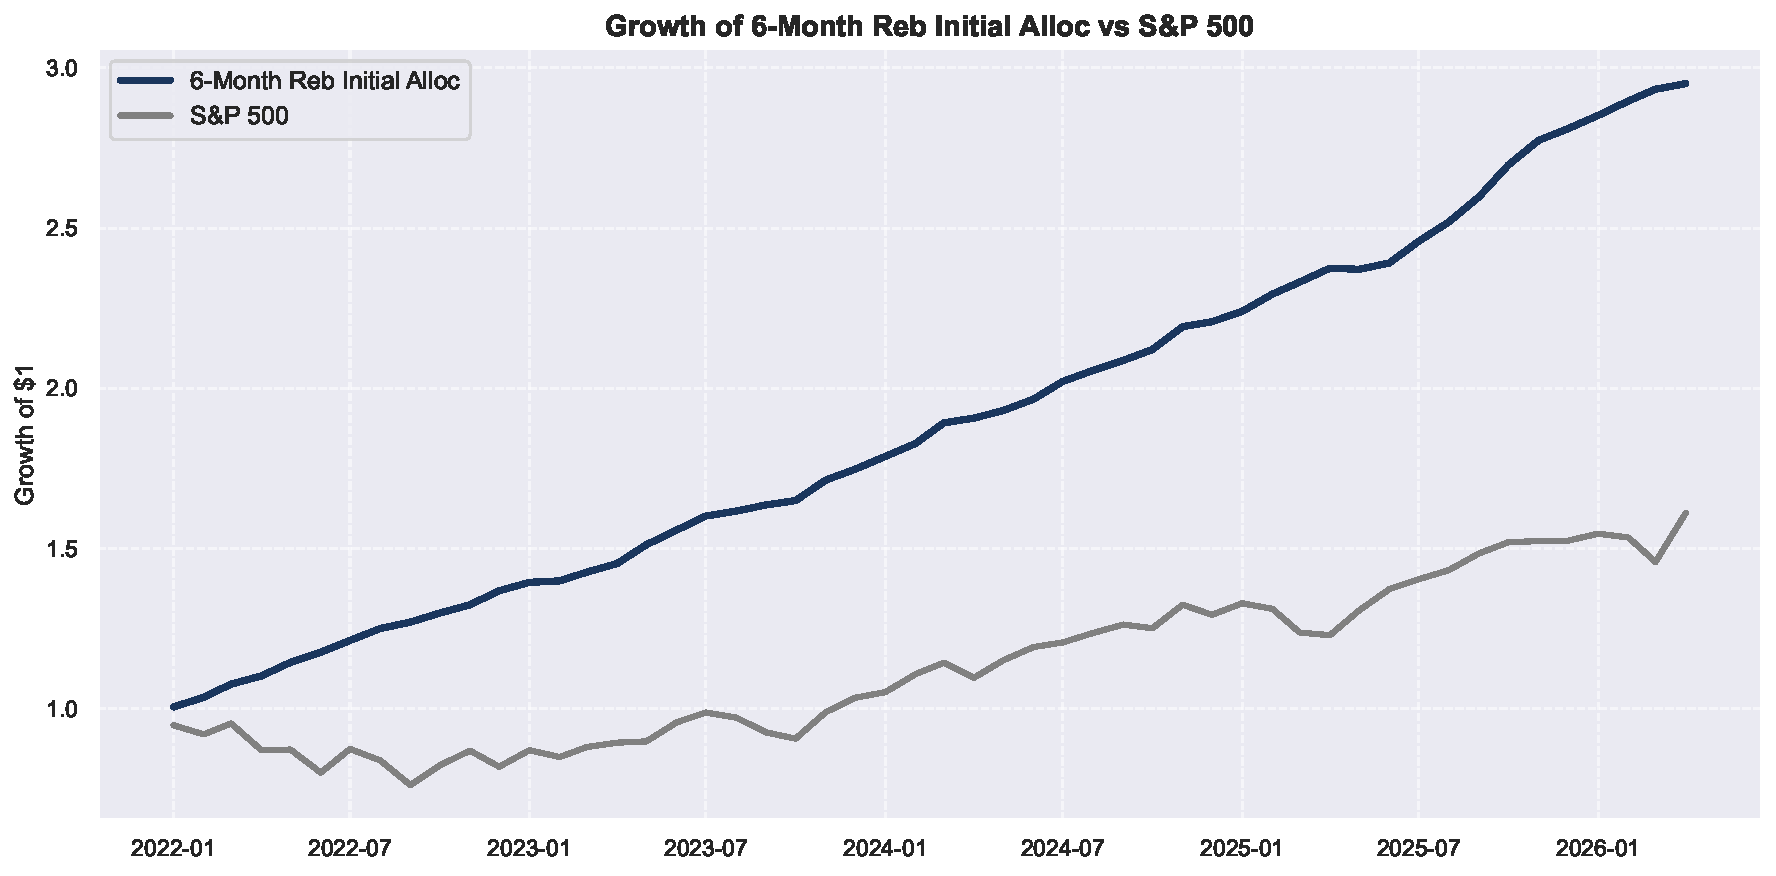
\includegraphics[width=0.9\textwidth]{growth_6_month_reb_initial_alloc_vs_sp500.pdf}
\end{figure}

\begin{figure}[h]
    \centering
    
\includegraphics[width=0.9\textwidth]{scatter_6_month_reb_initial_alloc_vs_sp500.pdf}
\end{figure}



\end{document}
